\documentclass{article}
\usepackage[utf8]{inputenc}

\title{SentinelMail: Benchmarking Multi-Model NLP Ensembles for Sensitive-Sentence Classification}
\author{Shelly Yaroslavsky (ID. 314982729), Erel Vanono (ID. 314804568)}
\date{Submitted as final project report for the NLP course, IDC, 2026}

\usepackage{natbib}
\usepackage{graphicx}

\begin{document}

\maketitle

\section{Introduction}

Sensitive-data leakage through organizational email is a long-standing
security challenge. With the growing adoption of generative AI,
sensitive information may also be exposed when users include personal,
financial, or confidential content in their interactions with AI
assistants. This new communication channel extends the traditional Data
Loss Prevention (DLP) problem and increases the need for reliable
detection of sensitive content in free-form text.

Sensitive information, however, does not have a uniform textual form.
Structured identifiers, such as credit-card numbers, social-security
numbers, and email addresses, often follow recognizable patterns. Other
disclosures may depend on linguistic context or appear in modified
formats; for example, the same phone number can be written as a
continuous sequence of digits or separated by spaces and hyphens.
Moreover, sensitive concepts may be mentioned in instructions,
negations, or hypothetical scenarios without revealing actual
information. These differences make it difficult for a single detection
approach to perform reliably across all forms of sensitive content.

In this work, we formulate sensitive-information detection as a
multi-label classification problem over short texts. Instead of
predicting only whether a text is sensitive, the system distinguishes
between benign content, general PII, financial information, and
confidential information. We evaluate four approaches with different
capabilities: a rule-based detector combining regular expressions and
named-entity recognition, a BiLSTM model with character-level
convolutional features, and two fine-tuned transformer classifiers
(BERT and RoBERTa). The rule-based detector focuses on known structured
patterns, the character-aware model captures variations in the internal
structure of sensitive tokens, and the transformers model the
linguistic context surrounding them.

While email DLP is the motivating application, we emphasize that it is
not the evaluated task. All quantitative results in this report are
obtained on the \texttt{ai4privacy/pii-masking-300k} dataset
\citep{ai4privacy2024}, a corpus
of short synthetic PII-bearing sentences. This text lacks the
characteristic structure of real email (subject lines, threading,
quoting, signatures), so our results measure sensitive-\emph{sentence}
classification and do not directly demonstrate performance on real
organizational email. We return to this external-validity limitation in
the Discussion.

Our study is organized around two research questions:

\begin{itemize}
    \item \textbf{RQ1:} Does a multi-model ensemble outperform the best
    single model for sensitive-content classification?
    \item \textbf{RQ2:} Does model complementarity vary across
    sensitivity categories (PII vs.\ financial vs.\ confidential)?
\end{itemize}

To answer these questions, we combine the four models into an ensemble.
Each model outputs a probability per sensitivity category, and the
ensemble averages these probabilities using a separate set of learned
weights for each category, so that a model can be trusted more for one
category and less for another. This weighting scheme is a standard
technique from the classifier-combination literature
\citep{kittler1998combining, kuncheva2004combining}, and we do not
present it as new. The contribution of this work lies elsewhere: the
learned weights, together with an ablation that removes one model at a
time, reveal which model each sensitivity category actually depends on,
and by how much. In other words, we use a standard ensemble to produce
an empirical map of model complementarity across sensitivity
categories.

\subsection{Related Work}

Sensitive-information detection has traditionally relied on regular
expressions, dictionaries, and named-entity recognition. These methods
are transparent and effective for structured identifiers, but their
dependence on predefined patterns limits their ability to recognize
context-dependent or irregular disclosures. Ahmed et al.\ demonstrated
the value of deep-learning methods for detecting context-dependent
sensitive information in unstructured text \citep{ahmed2021sensitive}.
Similarly, ExSense combined regular expressions for predictable
patterns with a BERT-BiLSTM-Attention model for context-based
sensitive-information extraction \citep{guo2021exsense}. Transformer
models \citep{devlin2019bert, liu2019roberta} have also shown strong
performance in sensitive-data detection and classification, including
BERT-based anonymization of clinical text \citep{garciapablos2020bert}.

Combining classifiers to exploit their complementary behavior is a
classical topic. Weighted soft voting and linear opinion pooling date
back to the multiple-classifier-systems literature
\citep{kittler1998combining}, and assigning a different combiner weight
per class is well established \citep{kuncheva2004combining}. More
expressive alternatives include stacked generalization
\citep{wolpert1992stacked} and mixture-of-experts gating
\citep{jacobs1991adaptive}. In multi-label settings, weighted ensemble
methods can assign different importance to individual classifiers for
different labels \citep{xia2021multilabel}. Our fusion rule is an
instance of per-class weighted soft voting; what we add is an empirical
comparison of pattern-aware, character-aware, and context-aware models
within a common sensitive-text classification framework, using the
learned per-category weights and ablations to characterize
complementarity across sensitivity categories.

\section{Methodology}
\label{sec:methodology}

\subsection{General Approach}
\label{subsec:general-approach}

The objective of this project is to develop a multi-label
sensitive-information detection system that benefits from the
complementary capabilities of different NLP approaches. Sensitive
information can appear as a recognizable structured pattern, an
irregular or obfuscated sequence, or a disclosure whose sensitivity
depends on the surrounding context. We therefore evaluate four models:
a rule-based detector, a BiLSTM with character-level features, and two
fine-tuned transformers (BERT and RoBERTa).

Given an input text, each model predicts whether it is benign and
whether it contains general personally identifiable information (PII),
financial information, or confidential information. Since the models
capture different textual signals, their predictions are subsequently
combined using category-specific confidence-weighted late fusion. The
complete solution consists of the following stages:

\begin{enumerate}
    \item \textbf{Data Preparation:}
    We load the English subset of the
    \texttt{ai4privacy/pii-masking-300k} dataset and derive
    text-level labels from its annotated sensitive entities.

    \item \textbf{Exploratory Data Analysis:}
    We examine label frequencies, label co-occurrence, entity
    distributions, and text lengths to understand the dataset and
    identify class imbalance.

    \item \textbf{Rule-Based Detection:}
    We use Microsoft Presidio and spaCy NER to detect sensitive
    information with recognizable patterns or known entity types.

    \item \textbf{Character-Aware Classification:}
    We train a BiLSTM model with character-level convolutional features
    to capture structural variations and obfuscated sensitive patterns.

    \item \textbf{Context-Aware Classification:}
    We fine-tune BERT and RoBERTa to classify sensitive content based
    on its linguistic context.

    \item \textbf{Category-Specific Fusion:}
    We combine the models' predictions using a separate set of weights
    for each sensitivity category, learned on a development split.

    \item \textbf{Evaluation and Analysis:}
    We compare the individual models and the ensemble using
    per-category metrics, confidence intervals, statistical
    significance testing, error analysis, and model ablation.
\end{enumerate}

\subsection{Data Preparation and Label Construction}
\label{subsec:data-preparation}

The dataset provides each text together with a \texttt{privacy\_mask}
containing the sensitive entities found in it. We convert these
entity-level annotations into a four-dimensional text-level label
vector:

\begin{equation}
    \mathbf{y}
    =
    \left[
        y_{\text{benign}},
        y_{\text{PII}},
        y_{\text{financial}},
        y_{\text{confidential}}
    \right].
    \label{eq:label-vector}
\end{equation}

A text is labeled as benign when it contains no annotated sensitive
entity. Any sensitive entity activates the PII label. Financial
identifiers (social-security numbers and card-related entities)
additionally activate the financial label, while passwords and
identity-document identifiers (passport, ID card, driver's licence)
activate the confidential label.

The labels have a hierarchical relationship. Financial and confidential
information are subsets of PII, while benign content is mutually
exclusive with all sensitive categories. A single text may therefore
belong to more than one sensitive category.

We note an important property of this construction: the labels are
\emph{derived} from the dataset's entity annotations rather than
independently annotated. The ground truth is therefore a deterministic
function of the entity mask, and part of what the models learn is to
recover this mapping. This is appropriate for comparing model families
on a shared task, but it should be kept in mind when interpreting
absolute scores, and it partly explains why pattern-based models are
competitive on categories defined by regex-shaped entities.

After filtering the dataset to English, the resulting data contain
29{,}908 training examples and 7{,}946 validation examples. To preserve
an untouched test set, we reserve the dataset's \texttt{validation}
split exclusively for final reporting (TEST) and carve a seeded 10\%
slice out of the training split (\texttt{train\_holdout}) to serve as
the development set (DEV) for model selection, ensemble-weight
learning, and threshold tuning. All models use the same preprocessing
and label-construction functions to ensure that their predictions are
evaluated against identical ground truth.

\subsection{Individual Models}
\label{subsec:individual-models}

\subsubsection{Rule-Based Detector}
\label{subsubsec:rule-based}

The rule-based detector represents the pattern-aware component of the
system. It uses Microsoft Presidio \citep{presidio}, which combines
regular-expression recognizers with spaCy named-entity recognition.

The detector identifies entities such as email addresses, phone
numbers, credit-card numbers, bank identifiers, social-security
numbers, passports, and driver's licences. Because stock Presidio has
no recognizers for several confidential entity types in our schema
(passwords, generic identity documents), we added three custom
recognizers covering password-like secrets, generic identity-document
numbers, and classification-marker vocabulary. The detected entities
are mapped to the project's four-label schema through the same entity
mapping used for ground-truth construction.

This model requires no training and provides transparent detections,
including the entity type, position, and confidence score. It is
expected to perform well on structured identifiers but to be less
effective when sensitive information is obfuscated, implicit, or
dependent on context.

\subsubsection{BiLSTM with Character-Level Features}
\label{subsubsec:bilstm}

The BiLSTM model represents the character-aware component. Each token
is represented using both a word embedding and a character-level
embedding. Word embeddings are initialized with pre-trained 100-dimensional
GloVe vectors \citep{pennington2014glove} and kept frozen during
training.

Character embeddings are passed through convolutional filters of
different sizes, allowing the model to learn local structural patterns
within words and identifiers. The resulting character representation is
concatenated with the word embedding and passed through a two-layer
bidirectional LSTM \citep{hochreiter1997lstm}.

The BiLSTM processes the text in both directions, and mean pooling is
applied across all non-padding positions. The pooled representation is
passed through a linear classification layer with four outputs. Sigmoid
activation converts these outputs into independent probabilities for
the four labels. The model is trained for 20 epochs with batch size 64
and learning rate $10^{-3}$, keeping the checkpoint with the best
validation loss.

This architecture is intended to recognize variations that fixed rules
may miss, including unusual separators, formatting changes, and tokens
that do not appear in a standard word vocabulary.

\subsubsection{Fine-Tuned Transformers: BERT and RoBERTa}
\label{subsubsec:transformers}

BERT \citep{devlin2019bert} and RoBERTa \citep{liu2019roberta}
represent the context-aware components of the system. Texts are
tokenized using each model's native tokenizer
(\texttt{bert-base-uncased} WordPiece and \texttt{roberta-base} BPE,
respectively) and truncated to a maximum of 512 tokens.

Both models use the contextual representation of the initial
classification token as a text-level representation. This
representation is passed through a linear classification layer that
produces four logits, which are converted into probabilities using
sigmoid activation.

To reduce computational cost, in both models the embedding layer and
the first ten transformer blocks are frozen; only the final two
transformer blocks and the classification head are fine-tuned. Training
uses binary cross-entropy with logits, positive-class weighting, label
smoothing, gradient clipping, and a learning-rate schedule with warmup.
Partial fine-tuning trades a small amount of accuracy for a
substantially smaller training footprint, which made the experiments
feasible on our hardware.

The transformers are intended to capture contextual information that
cannot be expressed through fixed patterns, including implicit
disclosures and mentions appearing in instructions, negations, or
hypothetical scenarios.

\subsection{Confidence-Weighted Late Fusion}
\label{subsec:fusion}

Each model produces a probability $p_{m,l}(x)$ for model $m$, label
$l$, and input text $x$. The ensemble combines these probabilities
separately for each label:

\begin{equation}
    p_{l}^{\text{ensemble}}(x)
    =
    \frac{
        \sum_{m} w_{m,l} \, p_{m,l}(x)
    }{
        \sum_{m} w_{m,l}
    },
    \label{eq:weighted-fusion}
\end{equation}

where $w_{m,l}$ represents the weight assigned to model $m$ for label
$l$.

Unlike uniform averaging, this formulation allows the same model to
have different importance across sensitivity categories. For example,
the rule-based detector may receive a larger weight for structured
financial information, while a transformer may receive a larger weight
for context-dependent PII. The BiLSTM may contribute more strongly when
sensitive information contains irregular character patterns.

The category-specific weights are fit on the DEV split by a per-label
grid search refined with Nelder--Mead optimization of the true
per-label F1. Per-label decision thresholds are tuned on the same DEV
split, and the identical tuned thresholds are then applied when
reporting on TEST. We deliberately chose this simple linear pooling
over more expressive alternatives such as stacking
\citep{wolpert1992stacked} or input-conditioned gating
\citep{jacobs1991adaptive}: with only four members, a linear pool with
per-category weights is less prone to overfitting the small development
split, and --- central to RQ2 --- the learned weights remain directly
interpretable as a measure of how much each category relies on each
model family.

\subsection{Evaluation Protocol}
\label{subsec:evaluation}

All models are evaluated using a shared evaluation framework on the
untouched TEST split. We report precision, recall, and F1 for each
sensitivity category, together with macro-F1 and ROC-AUC. Bootstrap
resampling (1{,}000 resamples, fixed seed) is used to estimate a 95\%
confidence interval for macro-F1. For RQ1, we additionally use a paired
bootstrap over TEST examples to test whether the ensemble's macro-F1
gain over the best single model is statistically significant, rather
than relying on point estimates alone. Model stability is assessed with
5-fold cross-validation.

In addition to aggregate metrics, we analyze false positives and false
negatives associated with negation, hypothetical language, implicit
disclosure, and obfuscated patterns. Since the dataset provides no
controlled contrast set for these phenomena, this analysis is
descriptive only and no robustness claim is attached to it. Finally, an
ablation study compares the complete ensemble with individual models
and leave-one-model-out configurations. Together with the learned
per-category weights, this analysis is used to answer RQ2: whether each
model provides a distinct contribution, and to which categories.

\subsection{Implementation and Process}
\label{subsec:implementation}

All models are implemented in Python with PyTorch and the HuggingFace
\texttt{transformers} library, and were trained on a single
Apple-Silicon machine using the MPS backend. Working on MPS required
two device-specific workarounds: disabling the fused
scaled-dot-product-attention fast path, which does not support the
attention-mask configuration used by our models, and reordering model
assembly relative to device placement to avoid an MPS memory-alignment
bug.

Beyond the code itself, the project followed an iterative internal
review process: an adversarial review pass over the methodology and
artifacts produced seventeen tracked issues, which led to concrete
changes --- among them the strict DEV/TEST split protocol described
above, consistent use of tuned thresholds at evaluation time, the
addition of significance testing for RQ1, and the honest descoping
decisions reported in the Introduction.

\section{Experimental results}
\label{sec:results}

\subsection{Settings}
\label{subsec:settings}

All numbers below are computed on the untouched TEST split (7{,}946
English examples). Ensemble weights and all decision thresholds were fit
on the DEV split (\texttt{train\_holdout}) and applied unchanged at test
time; the tuned per-label thresholds are 0.65 (benign), 0.40 (PII), and
0.50 (financial and confidential). Throughout this section,
\emph{headline macro-F1} averages F1 over the three informative
categories (PII, financial, confidential); \texttt{benign} is reported
per label but excluded from the macro, since it is the complement of PII
and would otherwise double-count the same decision. Confidence intervals
use bootstrap resampling (1{,}000 resamples, fixed seed).

\subsection{Main Comparison}
\label{subsec:main-comparison}

Table~\ref{tab:main-comparison} compares all systems under identical
thresholds and ground truth. A majority-prior baseline (predict the most
frequent label configuration) is included for orientation.

\begin{table}[t]
\centering
\small
\begin{tabular}{lccccc}
\hline
Model & benign & PII & financial & confid. & macro-F1 \\
\hline
Majority prior & 0.000 & 0.939 & 0.000 & 0.000 & 0.313 \\
Rule-based     & 0.605 & 0.943 & 0.656 & 0.807 & 0.802 \\
BiLSTM         & 0.835 & 0.975 & 0.915 & 0.951 & 0.947 \\
BERT           & 0.932 & 0.990 & 0.927 & 0.972 & 0.963 \\
RoBERTa        & 0.926 & 0.989 & 0.946 & 0.976 & \textbf{0.971} \\
Ensemble       & 0.934 & 0.991 & 0.946 & 0.975 & 0.970 \\
\hline
\end{tabular}
\caption{Per-label F1 and headline macro-F1 (PII/financial/confidential)
on TEST. 95\% bootstrap CIs for the two leading systems: RoBERTa
$[0.967, 0.974]$, ensemble $[0.967, 0.974]$.}
\label{tab:main-comparison}
\end{table}

The expected capability ordering holds: the rule-based detector is
strong on structured PII but weak where patterns are irregular or
contextual; the character-aware BiLSTM closes much of that gap; the two
transformers are strongest overall. The ensemble matches --- but does
not exceed --- the best single model. Per-label ROC-AUC for the ensemble
is 0.99 or higher for every category (macro AUC 0.993).

\paragraph{RQ1 verdict.} A paired bootstrap over TEST examples compares
the ensemble's headline macro-F1 (0.9703) against the best single model,
RoBERTa (0.9706). The delta is $-0.0003$ with 95\% CI
$[-0.0029, +0.0024]$ and $p = 0.80$: the difference is statistically
indistinguishable from zero. \textbf{The ensemble does not outperform
the best single model.} We treat this significance-gated negative result
as a finding, not a failure, and explain its mechanism below
(Section~\ref{subsec:why-no-gain}).

As a stability check, 5-fold cross-validation of the neural members
yields headline macro-F1 of $0.964 \pm 0.002$ (RoBERTa),
$0.959 \pm 0.003$ (BERT), and $0.941 \pm 0.006$ (BiLSTM), consistent
with the single-split ranking in Table~\ref{tab:main-comparison}.

\subsection{Per-Category Reliance (RQ2)}
\label{subsec:rq2}

Table~\ref{tab:weights} shows the learned fusion weights, and
Table~\ref{tab:ablation} the leave-one-member-out ablation.

\begin{table}[t]
\centering
\small
\begin{tabular}{lcccc}
\hline
Model & benign & PII & financial & confid. \\
\hline
BERT       & \textbf{0.70} & \textbf{0.80} & 0.20 & 0.00 \\
RoBERTa    & 0.10 & 0.00 & 0.00 & \textbf{0.51} \\
BiLSTM     & 0.10 & 0.10 & \textbf{0.50} & 0.39 \\
Rule-based & 0.10 & 0.10 & 0.30 & 0.10 \\
\hline
\end{tabular}
\caption{Learned per-category fusion weights (DEV-fit). Each column is
normalized at fusion time. Note the anomaly discussed in the text:
RoBERTa receives weight 0 on financial despite being the best single
financial model.}
\label{tab:weights}
\end{table}

\begin{table}[t]
\centering
\small
\begin{tabular}{lcccc}
\hline
Configuration & PII & financial & confid. & macro-F1 \\
\hline
Full ensemble        & 0.991 & 0.946 & 0.975 & 0.970 \\
$-$ BERT             & 0.969 & 0.936 & 0.975 & 0.960 \\
$-$ RoBERTa          & 0.991 & 0.946 & 0.953 & 0.963 \\
$-$ BiLSTM           & 0.990 & \textbf{0.656} & 0.975 & 0.874 \\
$-$ Rule-based       & 0.990 & 0.927 & 0.977 & 0.964 \\
RoBERTa alone        & 0.989 & 0.946 & 0.976 & 0.971 \\
\hline
\end{tabular}
\caption{Leave-one-member-out ablation on TEST (per-label F1 and
headline macro-F1).}
\label{tab:ablation}
\end{table}

Reliance is clearly category-differential: removing BERT hurts PII
($0.991 \rightarrow 0.969$), removing RoBERTa hurts confidential
($0.975 \rightarrow 0.953$), and removing the BiLSTM collapses financial
($0.946 \rightarrow 0.656$). So the answer to RQ2 is yes --- the fitted
ensemble leans on different members for different categories.

However, this reliance must not be over-read as intrinsic model
complementarity, because it is confounded by the weight-fitting
procedure. The clearest symptom is financial: the fit assigned RoBERTa a
weight of exactly 0 (Table~\ref{tab:weights}) even though RoBERTa alone
is the \emph{best} single financial model (F1 $= 0.946$,
Table~\ref{tab:ablation}). The ensemble therefore carries financial on
BiLSTM, BERT, and the rule-based detector; dropping the BiLSTM
renormalizes onto the weaker remaining members and the score collapses.
The collapse demonstrates sensitivity to a quirky weight fit --- not
that RoBERTa needs the BiLSTM. Read honestly, RQ2's finding is ``the
fitted ensemble depends on different members per category,'' which is
weaker than ``the models intrinsically complement each other,'' and it
does not translate into a net gain over the best single model (RQ1).

\subsection{Why the Ensemble Cannot Win}
\label{subsec:why-no-gain}

Two measurements explain the null RQ1 result mechanistically.

\paragraph{Oracle ceiling.} For each category we compute the accuracy of
an oracle that, per example, selects whichever member happens to be
correct --- an upper bound on any per-example combiner. The best single
model already sits within 1.2--1.7 accuracy points of this ceiling: PII
0.982 vs.\ oracle 0.994, financial 0.979 vs.\ 0.993, confidential 0.978
vs.\ 0.995. With so little headroom, even a perfect combiner could only
match the best member, not meaningfully pass it. (The oracle bound is
computed in accuracy space while the headline metric is F1, so it is a
headroom proxy rather than an exact F1 ceiling; the qualitative
conclusion is robust.)

\paragraph{Correlated errors.} Figure~\ref{fig:error-overlap} shows the
pairwise Jaccard overlap of the members' error sets. The two
transformers make largely the same mistakes (overlap 0.41 on PII, 0.39
on financial, 0.48 on confidential), while the rule-based detector is
the most decorrelated member but also the weakest. Ensembles profit from
diverse errors among comparably strong members; here the strong members
agree and the diverse member is weak.

\begin{figure}[t]
\centering
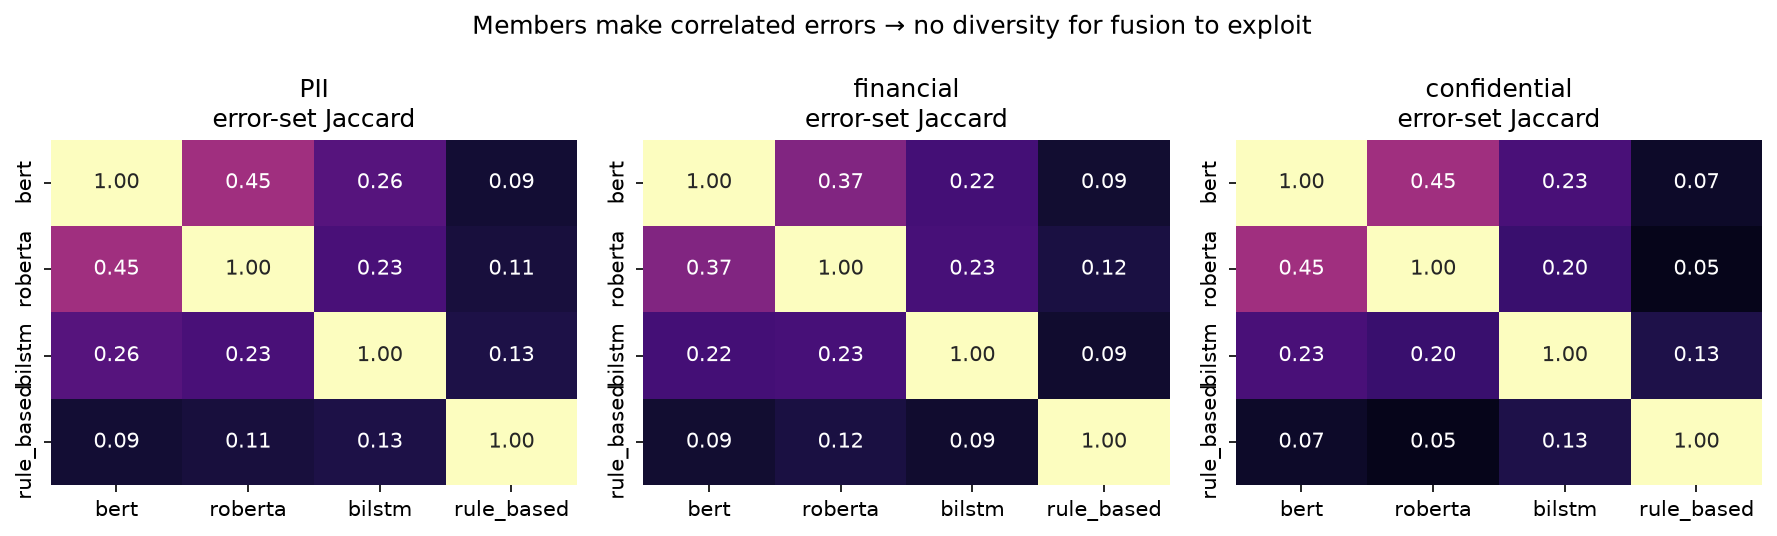
\includegraphics[width=\linewidth]{figures/error_overlap.png}
\caption{Pairwise Jaccard overlap of member error sets per category.
High transformer--transformer overlap leaves little diversity for the
ensemble to exploit.}
\label{fig:error-overlap}
\end{figure}

\subsection{DLP Operating Point}
\label{subsec:operating-point}

Headline macro-F1 uses F1-optimal thresholds, but a deployed DLP system
runs at high recall, since a missed sensitive item costs far more than a
false alarm. Figure~\ref{fig:pr-curves} shows the ensemble's
precision--recall curves per category. At a recall floor of 0.99, the
ensemble attains the best
per-category precision of any system: 0.467 (benign), 0.993 (PII), 0.647
(financial), 0.960 (confidential), each at least matching the best
single model (e.g., RoBERTa reaches 0.620 on financial and 0.954 on
confidential at the same floor). Three caveats keep this a hint rather
than a reversal of RQ1: the thresholds meeting the recall floor are
selected on the TEST split itself, so these are optimistic upper bounds;
the edge is not significance-tested; and the benign and financial values
sit in low-precision regions where estimates are noisy.

\begin{figure}[t]
\centering
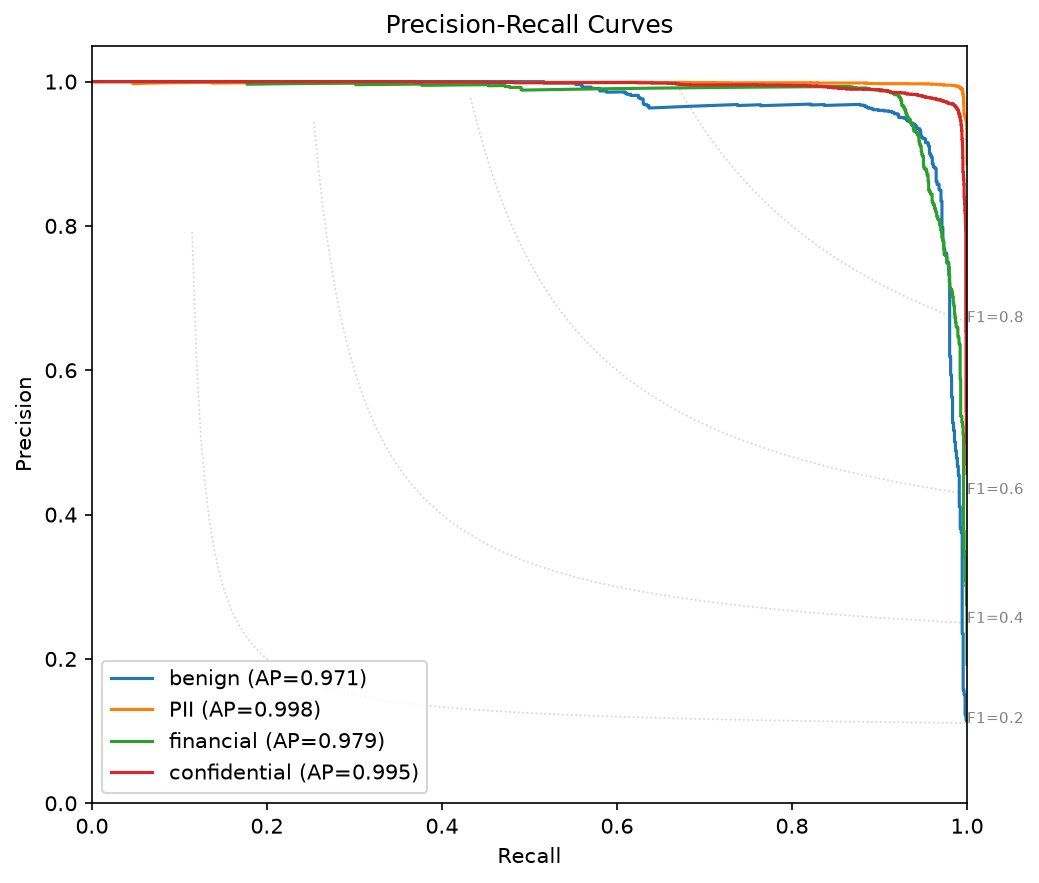
\includegraphics[width=\linewidth]{figures/pr_curves_novelty.png}
\caption{Ensemble precision--recall curves per category on TEST (dotted
lines are iso-F1 contours). DLP deployment operates at the far right of
these curves (recall $\geq 0.99$), where the benign and financial curves
drop steeply.}
\label{fig:pr-curves}
\end{figure}

\subsection{Error Analysis and Efficiency}
\label{subsec:error-analysis}

A descriptive pass over the strongest single model's TEST errors sorts
them into negation, hypothetical, implicit-disclosure, and obfuscation
buckets. False positives concentrate in negation-framed benign mentions
of sensitive concepts, and the residual false negatives include
obfuscated identifiers and implicit disclosures; the majority of errors,
however, fall outside all four buckets. Because the dataset provides no
controlled contrast set for these phenomena, this analysis remains
descriptive and no robustness claim is attached to it.

Finally, the efficiency accounting is one-sided: the ensemble evaluates
every member at inference time ($\approx$241M parameters, dominated by
the two transformers) versus $\approx$125M for RoBERTa alone ---
roughly twice the compute for a macro-F1 delta indistinguishable from
zero. On this dataset, deploying the ensemble is not justified.

\section{Discussion}
\label{sec:discussion}

\paragraph{RQ1: no.} On this dataset, a per-category weighted ensemble
of four heterogeneous models does not outperform a single fine-tuned
RoBERTa: the macro-F1 delta is $-0.0003$ with a 95\% CI spanning zero
($p = 0.80$). We consider this significance-gated negative result the
central finding of the project, and the more informative because a
per-category ensemble is exactly what a practitioner would naturally
reach for. The mechanism is clear: the best single model already sits
within 1.7 accuracy points of the per-example oracle ceiling, and the
strongest members make largely the same mistakes. With that little
headroom and that much error correlation, no combiner --- ours or a more
expressive one --- had room to help. When a strong fine-tuned
transformer is available, late fusion adds nothing on this task; the
2$\times$ inference cost buys a delta indistinguishable from zero.

\paragraph{RQ2: yes, with a confound.} The fitted ensemble does lean on
different members per category --- BERT for PII, the BiLSTM for
financial, RoBERTa for confidential --- and the ablation confirms that
removing a member hurts precisely the category it is weighted for. But
the reliance is a property of the fitted weights, not proof of intrinsic
complementarity: the fit zero-weighted RoBERTa on financial despite
RoBERTa being the best single financial model, which both explains the
dramatic financial collapse when the BiLSTM is removed and leaves the
ensemble marginally worse on financial than RoBERTa alone. A refit that
guarantees RoBERTa a financial weight would test whether the reliance
pattern survives; we flag this as follow-up work. The one place the
ensemble shows an edge --- best per-category precision at the
recall~$\geq 0.99$ operating point --- is reported with its caveats
(test-split thresholds, no significance test) as a hint for future work
rather than a result.

\paragraph{Limitations.} All results are on synthetic, sentence-level
PII text; nothing here demonstrates performance on real organizational
email (no subject lines, threading, or email register), and an email
domain-shift evaluation is the most valuable next step. Labels are
derived deterministically from the dataset's entity mask, so absolute
scores ($\approx$0.97) partly reflect models recovering a known mapping
on an easy synthetic task. The per-category weights were fit on a
development split with limited support for the rarer categories, which
plausibly contributed to the degenerate financial fit. The oracle bound
is computed in accuracy space, a proxy for the F1 headline. Finally, as
described in the Introduction, the health label, a zero-shot-LLM
comparison, and a controlled robustness study were descoped; the error
buckets we report are descriptive only.

\paragraph{Process insights.} Several of this project's conclusions were
made trustworthy by protocol fixes found during internal adversarial
review rather than by modeling work: reserving an untouched TEST split
after discovering the original selection split had been reused for
tuning; applying tuned thresholds consistently to every system rather
than mixing threshold conventions across tables; excluding the benign
complement label from the headline macro; and gating the ensemble claim
on a paired significance test instead of a point-estimate comparison
(which, under the earlier flawed conventions, had shown an apparent
ensemble ``win''). The transferable methodological takeaway: confirm an
ensemble claim with an ablation \emph{and} a significance test, and
judge it at the operating point the application will actually use.

\section{Code}

The complete implementation --- data preparation, the four models, the
fusion and evaluation packages, notebooks 01--07 (data exploration, one
notebook per model, ensemble training, and the novelty analysis that
generates every number and figure in Section~\ref{sec:results}), and all
result artifacts --- is available at:
% TODO: insert repository link once the submission location is decided.
\texttt{<repository link>}.

\bibliographystyle{plain}
\bibliography{references}
\end{document}
